\documentclass[oneside,a4paper]{report}
\usepackage{color}
\usepackage{longtable}
\usepackage{titlesec}
\usepackage[hidelinks]{hyperref}
\usepackage{ulem}
\usepackage{graphicx}
\usepackage{fancyhdr}
\usepackage[T1]{fontenc}
\usepackage[headheight=25pt,margin=0.7in,top=1.5in,bottom=1in,right=1in,left=1in]{geometry}

\hypersetup{colorlinks=true,linktoc=none,citecolor=black,urlcolor=blue}
\hypersetup{linktocpage=false,linkcolor=black}

\pagestyle{fancy}
\fancyhead[R]{
\includegraphics[width=2cm]{./latex/resources/kitlogo.png}}
\fancyhead[L]{\leftmark}

\fancypagestyle{plain}{
        \rhead{
\includegraphics[width=2cm]{./latex/resources/kitlogo.png}}
        \lhead{\leftmark}
}


\renewcommand{\arraystretch}{2}

\titleformat{\chapter}[hang]
 {\normalfont\bfseries\LARGE}{\thechapter. }{0pt}{\LARGE}
\titleformat{\section}[hang]
 {\normalfont\bfseries\Large}{\thesection. }{0pt}{\Large}
\titleformat{\paragraph}[hang]
 {\normalfont\bfseries\normalsize}{}{}{}

\titlespacing*{\chapter}{0pt}{-20pt}{10pt}

\begin{document}
  \begin{titlepage}
	\centering
	{\scshape\LARGE Karlsruhe Institute of Technology \par}
	\vspace{1cm}
	{\scshape\Large Software Engineering Practice\par}
	\vspace{0.5cm}
	{\scshape\Large WINTER TERM 2015/2016\par}
	\vspace{1.5cm}
	{\Huge\bfseries rootJS - module guide\par}
	\vspace{0.25cm}
	{\Large\bfseries Node.js bindings for ROOT 6\par}
	\vspace{2cm}
	{\Large\itshape Jonas Schwabe\par}
	{\Large\itshape Theo Beffart\par}
	{\Large\itshape Sachin Rajgopal\par}
	{\Large\itshape Christoph Wolff\par}
	{\Large\itshape Christoph Haas\par}

	{\Large\itshape Maximilian Fr\"uh\par}
	\vfill
	supervised by\par
	Dr.~Marek \textsc{Szuba}

	\vfill

	% Bottom of the page
	{\large \date{99.99.9999}\par}
\end{titlepage}

  \tableofcontents
  \clearpage
  %\input{./latex/purpose.tex}
  \chapter{NodeApplication}
describe class NodeApplication here
\section{NodeApplication}
\begin{longtable}{p{3cm} @{\hskip 1cm} p{12cm}}
 \hline
\textit{Name} & \texttt{NodeApplication::NodeApplication(acn: char*, argc: int*, argv: char**)}\\
\hline
 \textit{Visibility} & public\\
\hline
\textit{Parameters} & \textit{acn: char*, argc: int*, argv: char**}\\
\hline
\textit{Return value} & \textbf{ <<constructor>>} describe return value\\
  \hline
 \textit{Behavior} & describe beahviour \\
\hline
\end{longtable} \pagebreak
 
  \chapter{CallbackHandler}
The CallbackHandler class gets invoked whenever an encapsulated ROOT function or object is accessed.
\section{ctorCallback}
\begin{longtable}{p{3cm} @{\hskip 1cm} p{12cm}}
 \hline
\textit{Name} & \texttt{CallbackHandler::ctorCallback(args: FunctionCallbackInfo<Value>)}\\
\hline
 \textit{Visibility} & public\\
\hline
\textit{Parameters} & \textit{args: FunctionCallbackInfo<Value>} information about the context\\
\hline
\textit{Return value} & \textbf{none}\\
  \hline
 \textit{Behavior} & Gets invoked whenever a non static constructor function of an encapsulated ROOT class was called.\\
\hline
\end{longtable} \pagebreak
 \section{staticCtorCallback}
\begin{longtable}{p{3cm} @{\hskip 1cm} p{12cm}}
 \hline
\textit{Name} & \texttt{CallbackHandler::staticCtorCallback(args: FunctionCallbackInfo<Value>)}\\
\hline
 \textit{Visibility} & public\\
\hline
\textit{Parameters} & \textit{args: FunctionCallbackInfo<Value>}\\
\hline
\textit{Return value} & \textbf{none}\\
  \hline
 \textit{Behavior} & Gets invoked whenever a static constructor of an encapsulated ROOT class was called.\\
\hline
\end{longtable} \pagebreak
 \section{memberGetterCallback}
\begin{longtable}{p{3cm} @{\hskip 1cm} p{12cm}}
 \hline
\textit{Name} & \texttt{CallbackHandler::memberGetterCallback(property: Local<String>, info: PropertyCallbackInfo<Value>)}\\
\hline
 \textit{Visibility} & public\\
\hline
\textit{Parameters} & \textit{property: Local<String>, info: PropertyCallbackInfo<Value>}\\
\hline
\textit{Return value} & \textbf{none}\\
  \hline
 \textit{Behavior} & Gets invoked whenever an encapsulated (class) member was requested.\\
\hline
\end{longtable} \pagebreak
 \section{memberSetterCallback}
\begin{longtable}{p{3cm} @{\hskip 1cm} p{12cm}}
 \hline
\textit{Name} & \texttt{CallbackHandler::memberSetterCallback(property: Local<String>, value: Local<Value>, info: PropertyCallbackInfo<Value>)}\\
\hline
 \textit{Visibility} & public\\
\hline
\textit{Parameters} & \textit{property: Local<String>, value: Local<Value>, info: PropertyCallbackInfo<Value>}\\
\hline
\textit{Return value} & \textbf{none}\\
  \hline
 \textit{Behavior} & Gets invoked whenever an encapsulated (class) member is attempted to be set.\\
\hline
\end{longtable} \pagebreak
 \section{memberFunctionCallback}
\begin{longtable}{p{3cm} @{\hskip 1cm} p{12cm}}
 \hline
\textit{Name} & \texttt{CallbackHandler::memberFunctionCallback(args: FunctionCallbackInfo<Value>)}\\
\hline
 \textit{Visibility} & public\\
\hline
\textit{Parameters} & \textit{args: FunctionCallbackInfo<Value>}\\
\hline
\textit{Return value} & \textbf{none}\\
  \hline
 \textit{Behavior} & Gets invoked whenever an non-static (class) function was called.\\
\hline
\end{longtable} \pagebreak
 \section{staticGetterCallback}
\begin{longtable}{p{3cm} @{\hskip 1cm} p{12cm}}
 \hline
\textit{Name} & \texttt{CallbackHandler::staticGetterCallback(property: Local<String>, info: PropertyCallbackInfo<Value>)}\\
\hline
 \textit{Visibility} & public\\
\hline
\textit{Parameters} & \textit{property: Local<String>, info: PropertyCallbackInfo<Value>}\\
\hline
\textit{Return value} & \textbf{none}\\
  \hline
 \textit{Behavior} &  Gets invoked whenever an encapsulated static object was requested.\\
\hline
\end{longtable} \pagebreak
 \section{staticSetterCallback}
\begin{longtable}{p{3cm} @{\hskip 1cm} p{12cm}}
 \hline
\textit{Name} & \texttt{CallbackHandler::staticSetterCallback(property: Local<String>, value: Local<Value>, info: PropertyCallbackInfo<Value>)}\\
\hline
 \textit{Visibility} & public\\
\hline
\textit{Parameters} & \textit{property: Local<String>, value: Local<Value>, info: PropertyCallbackInfo<Value>}\\
\hline
\textit{Return value} & \textbf{none}\\
  \hline
 \textit{Behavior} & Gets invoked whenever an encapsulated static object is attempted to be set.\\
\hline
\end{longtable} \pagebreak
 \section{staticFunctionCallback}
\begin{longtable}{p{3cm} @{\hskip 1cm} p{12cm}}
 \hline
\textit{Name} & \texttt{CallbackHandler::staticFunctionCallback(args: FunctionCallbackInfo<Value>)}\\
\hline
 \textit{Visibility} & public\\
\hline
\textit{Parameters} & \textit{args: FunctionCallbackInfo<Value>}\\
\hline
\textit{Return value} & \textbf{none}\\
  \hline
 \textit{Behavior} & Gets invoked whenever a static function was called.\\
\hline
\end{longtable} \pagebreak

  \chapter{ProxyObjectFactory}
describe class ProxyObjectFactory here
\section{createProxyObject}
\begin{longtable}{p{3cm} @{\hskip 1cm} p{12cm}}
 \hline
\textit{Name} & \texttt{ProxyObjectFactory::createProxyObject(type: TDataMember, scope: TClassRef, holder: ProxyObject)}\\
\hline
 \textit{Visibility} & public\\
\hline
\textit{Parameters} & \textit{type: TDataMember, scope: TClassRef, holder: ProxyObject}\\
\hline
\textit{Return value} & \textbf{ ProxyObject} describe return value\\
  \hline
 \textit{behavior} & describe beahviour \\
\hline
\end{longtable} \pagebreak
 
  \chapter{ProxyObject}
ProxyObject is an interace defining the following abstract methods:
\section{isScalar}
\begin{longtable}{p{3cm} @{\hskip 1cm} p{12cm}}
  \hline
  \textit{Name} & \texttt{ProxyObject::isScalar())} \\
  \hline
  \textit{Visibility} & Public abstract \\
  \hline
  \textit{Parameters} & \textit{none} \\
  \hline
  \textit{Return value} & \textbf{bool} true: The object is scalar, no recursion is needed to create a ROOT/v8 representation \\
  \hline
  \textit{behavior} & This is usually just a return statement, as String, Number, Bool, ... ProxyObjects will always handle scalar data and ObjectProxyObjets will be the only non scalar ProxyObjects (and will therefor return false) \\
  \hline
\end{longtable}
\section{getV8Handle}
\begin{longtable}{p{3cm} @{\hskip 1cm} p{12cm}}
  \hline
  \textit{Name} & \texttt{ProxyObject::getV8Handle())} \\
  \hline
  \textit{Visibility} & Public abstract \\
  \hline
  \textit{Parameters} & \textit{none} \\
  \hline
  \textit{Return value} & \textbf{v8::Handle} A Handle will be generated continaing the data, used to initialize the ProxyObject. \\
  \hline
  \textit{behavior} & This highly depends on the obecjt's type scalar types might just call a constructor and return the result, ObjectProxyObjects will need to step down all through the objects children. \\
  \hline
\end{longtable}

  \chapter{ProxyObjectCache}
The ProxyObjectCache is a key value store, mapping memory addresses to V8 or ROOT objects.

Some sort of cache is essential in this case, because we might need to deal with cyclic dependencies which would lead to an endless recursion in the ProxyObjectFactory.
Using a cache would make cyclic references easy to handle. During conversion of an object it's content must not change so that the cache is valid, after the conversion, the whole cache should be considered dirty because we cannot monitor all changes in either ROOT's nor node's data.

Invalidating the cache after each conversion means that there is more or less no performance gain, in most cases, when we only have linear references, there are only objects written to the cache without any cache hit before invalidation.
\\
\textbf{IDEA:} Make the cache locally instead of globally available, so that instead of invalidate it, we reinitialize it.
\section{invalidate}
\begin{longtable}{p{3cm} @{\hskip 1cm} p{12cm}}
  \hline
  \textit{Name} & \texttt{ProxyObjectCache::invalidate()} \\
  \hline
  \textit{Visibility} & Public \\
  \hline
  \textit{Parameters} & \textit{none} \\
  \hline
  \textit{Return value} & \textit{none} \\
  \hline
  \textit{behavior} & Clears (or invalidates) the whole cache, so that a cache query does not have a hit, even if it has been mapped before the invalidate call \\
  \hline
\end{longtable}
\newpage
\section{put}
\begin{longtable}{p{3cm} @{\hskip 1cm} p{12cm}}
  \hline
  \textit{Name} & \texttt{ProxyObjectCache::put(long key, void value)} \\
  \hline
  \textit{Visibility} & Public \\
  \hline
  \textit{Parameters} & \textbf{key}: is the key which should refer to value, \textbf{value}: is the value to be cached\\
  \hline
  \textit{Return value} & \textit{none} \\
  \hline
  \textit{behavior} & Stores the value in the cache and makes it available so that value == cache->get(key) is true after this call \\
  \hline
\end{longtable}
\newpage
\section{get}
\begin{longtable}{p{3cm} @{\hskip 1cm} p{12cm}}
  \hline
  \textit{Name} & \texttt{ProxyObjectCache::get(long key)} \\
  \hline
  \textit{Visibility} & Public \\
  \hline
  \textit{Parameters} & \textit{none} \\
  \hline
  \textit{Return value} & \textbf{void}: the value mapped to the given key \\
  \hline
  \textit{behavior} & Returns the value that is related to the given key, if the entry is still valid \\
  \hline
\end{longtable}

  \chapter{Appendix}
\section{Class diagram} % Object Model

\begin{figure}[htb]
	\centering
	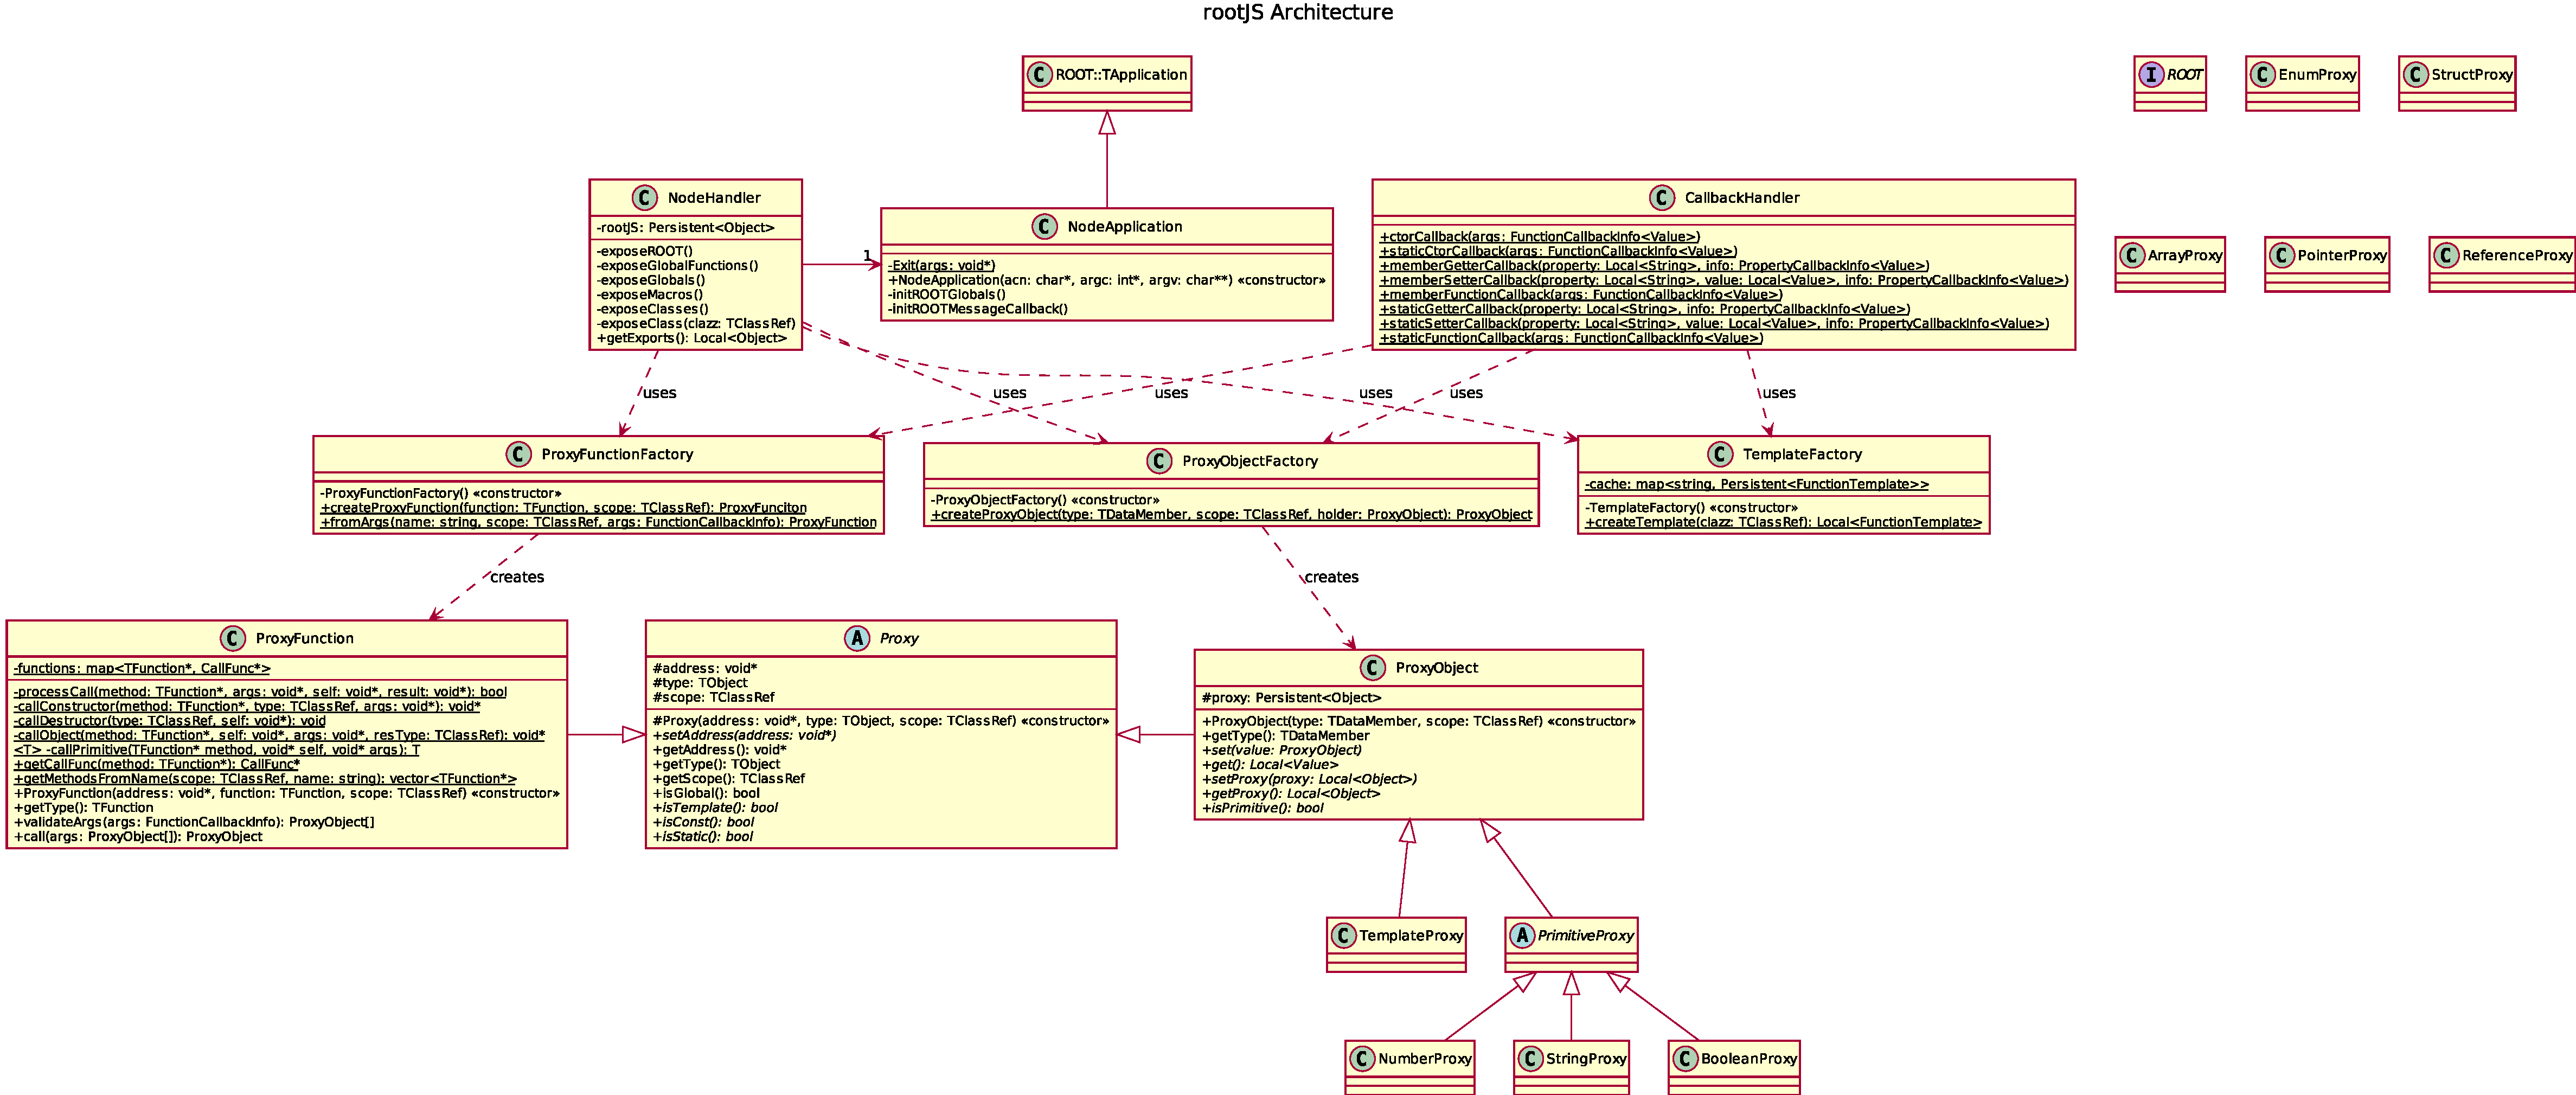
\includegraphics[width=\textheight, height=\linewidth, angle={90}, keepaspectratio]{./latex/resources/architecture.pdf}
	\caption{rootJS class diagram}
\end{figure}

\pagebreak

\section{Dynamic Model}

\begin{figure}[htb]
	\centering
	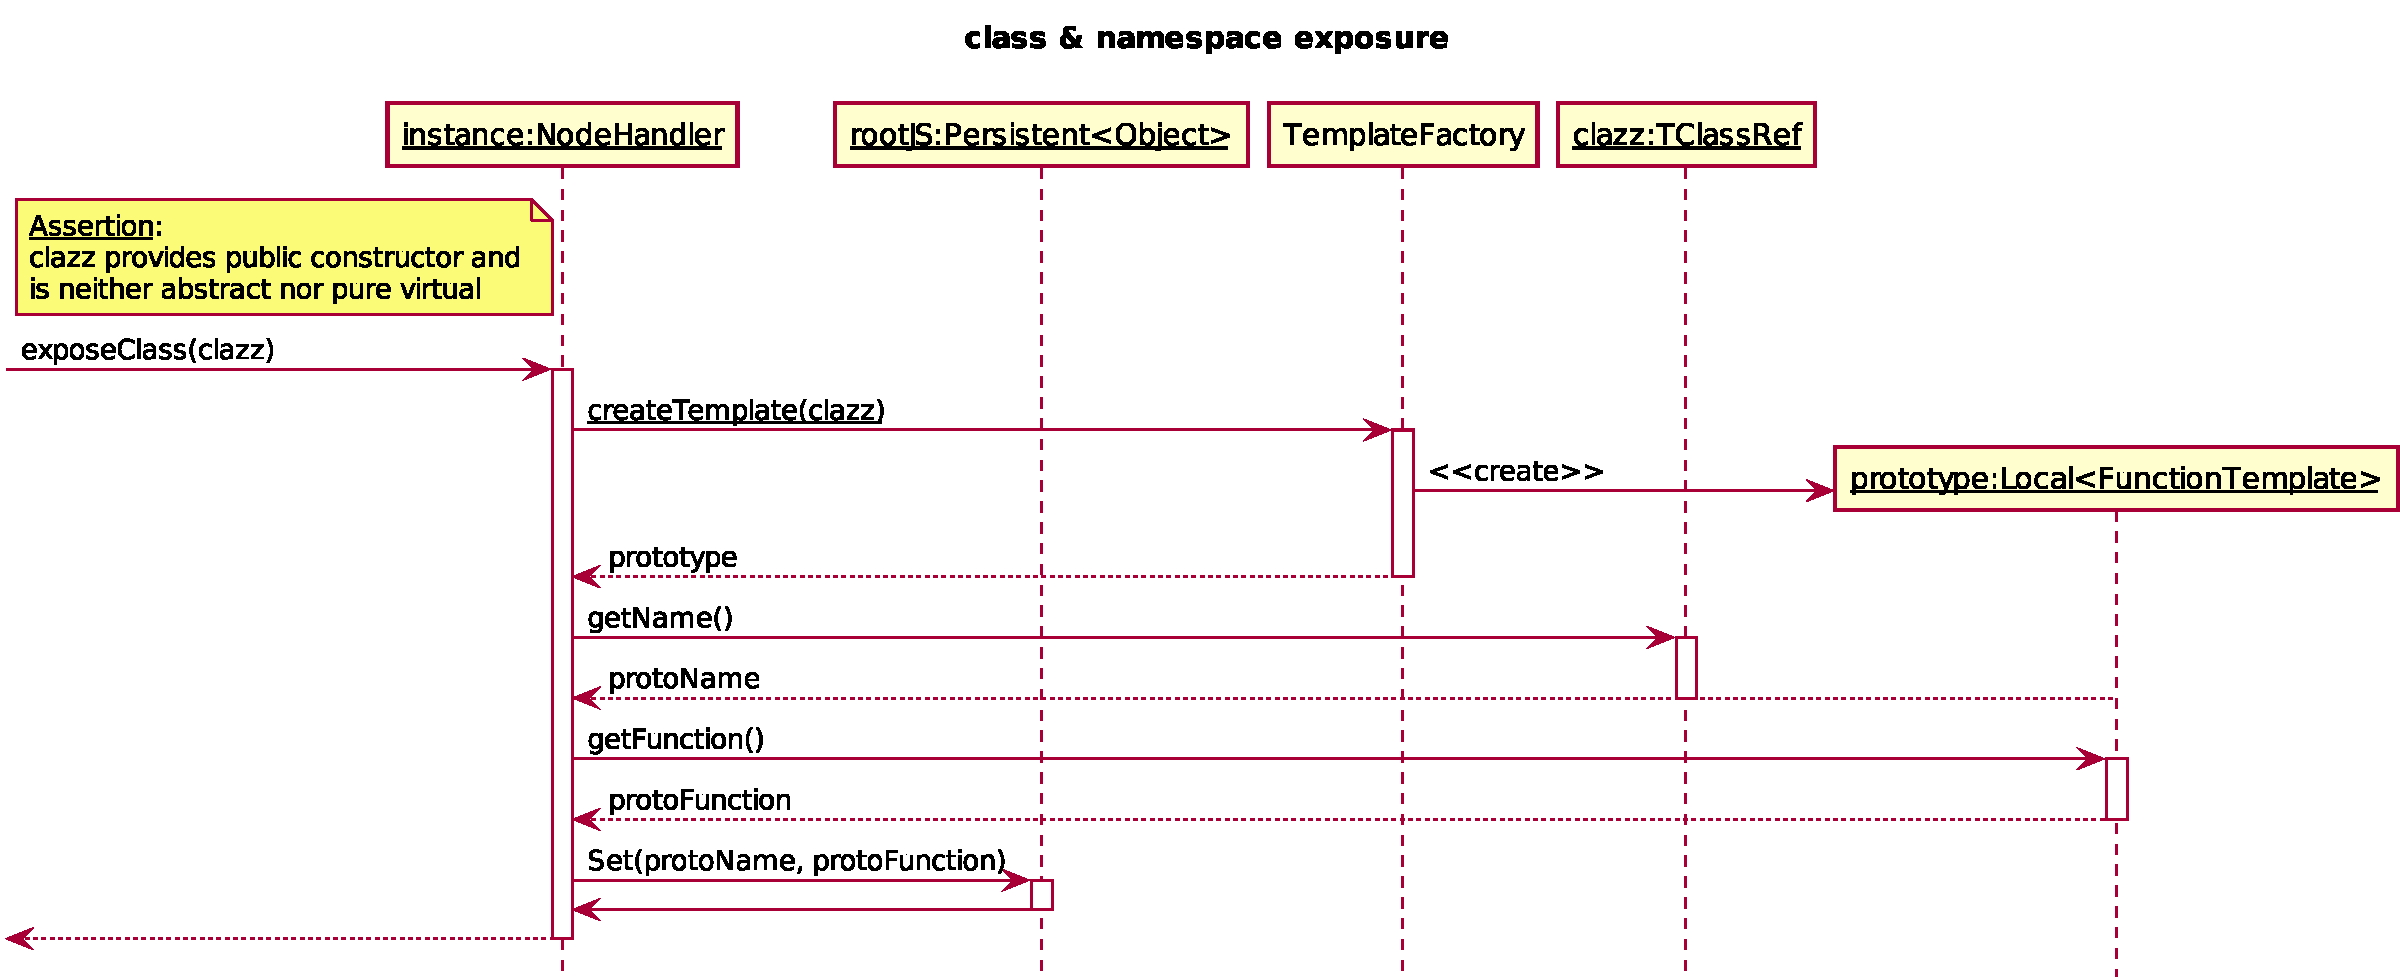
\includegraphics[width=18cm]{./latex/resources/classExposureSequence.pdf}
	\caption{class exposure sequence}
\end{figure}

\begin{figure}[htb]
	\centering
	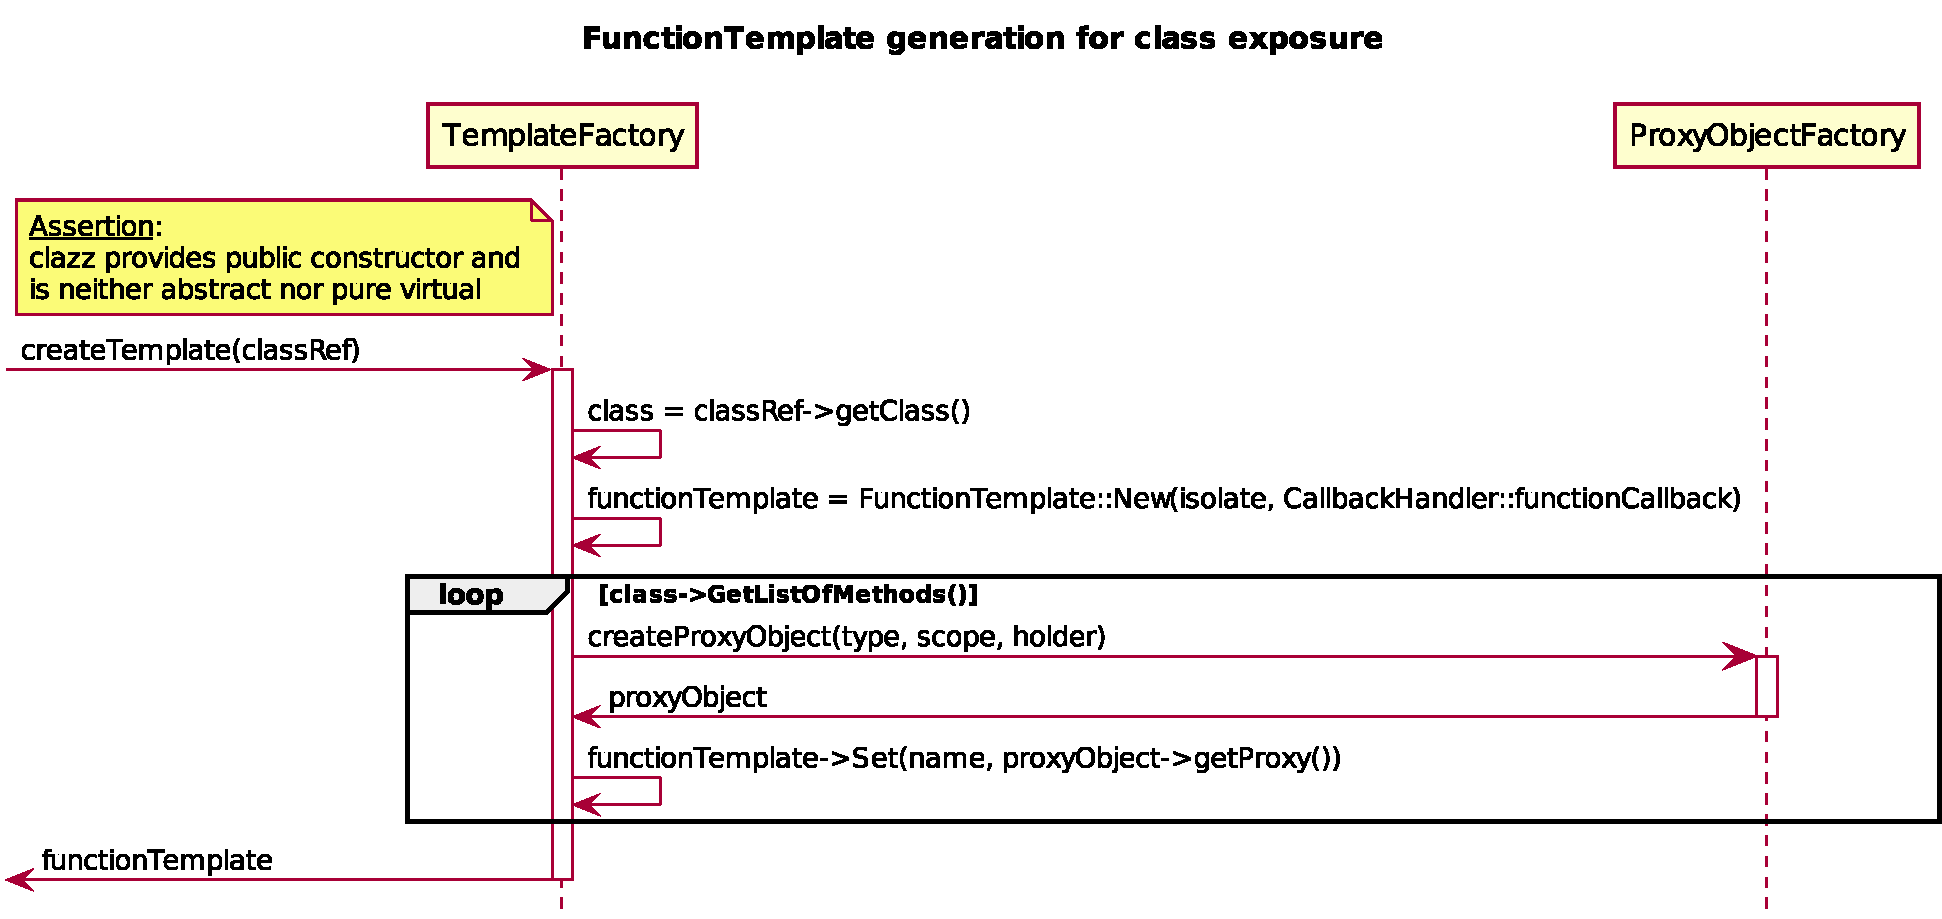
\includegraphics[width=18cm]{./latex/resources/functionTemplateGenerate.pdf}
	\caption{class exposure sequence}
\end{figure}

\begin{figure}[htb]
	\centering
	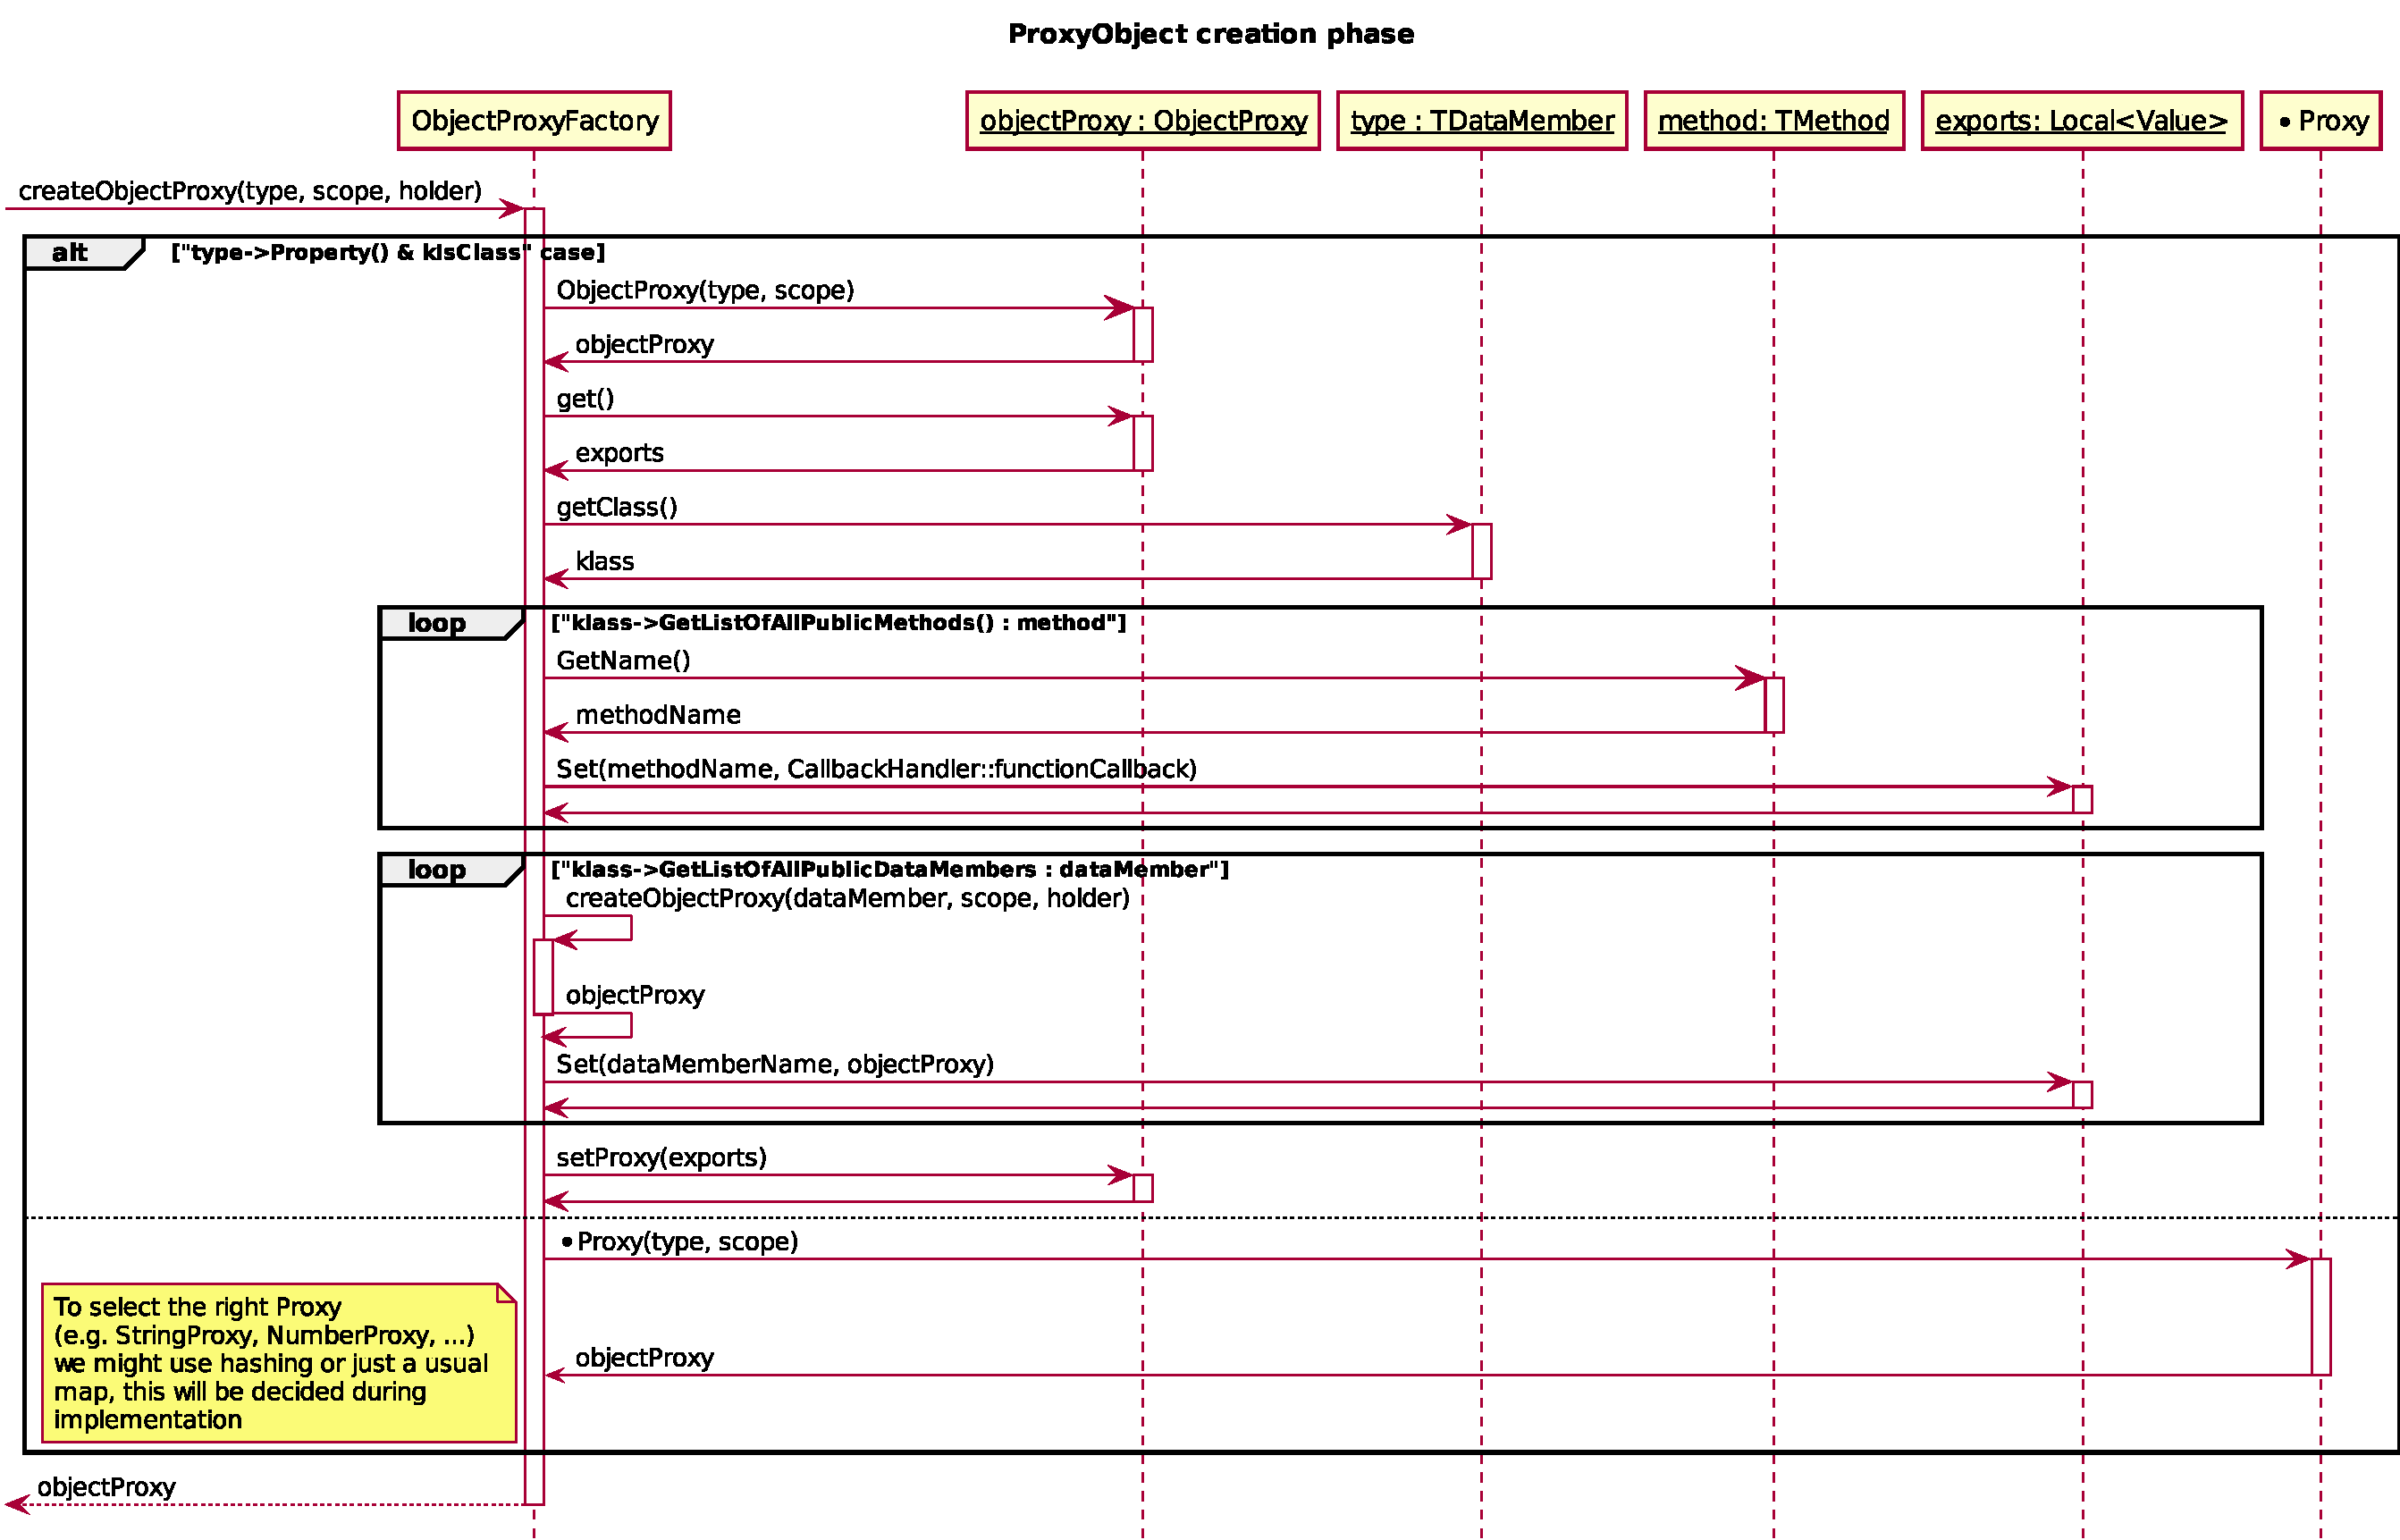
\includegraphics[width=18cm]{./latex/resources/createProxyObject.pdf}
	\caption{ProxyObject creation sequence}
\end{figure}

\newpage

\section{Glossary}
\paragraph{Callback}
A function which is passed as an argument to some code, which is then expected to call the argument back.
\paragraph{Constructor}
A method which is used to create an object.
\paragraph{Encapsulation}
A piece of functionality of certain languages used to restrict access to some of the object's variables and methods
\paragraph{Instance}
A created object.
\paragraph{Proxy}
A class functioning as an intermediary between two classes.
\paragraph{Static}
A method which does not require the object to be instantiated.
\paragraph{Template} 
A feature of C++ that allows classes and functions to operate with generic types.
\paragraph{v8} 
An open source JavaScript engine, written in C++ and made by Google.

\newpage




\end{document}
